\section{Methodology}
\label{sec:meth}
Within this research the final goal is to construct a classifier which is able to classify municipality documents correctly. In order to do this, a multitude of algorithms are examined. Also, the influence of the domain adaptivity and importance sampling are researched. This section introduces the datasets, experiments and further detail about the implementation of the algorithms.

\subsection{Description of the data}
\label{subsec:data}
Two datasets have been used within this research which both include documents from the government of the Netherlands. The first set, called PAR\_ALL, consists of over 50,000 questions and answers that have been asked within the Dutch national parliament during 2001-2017 and these questions were scraped from www.zoek.officielebekendmakingen.nl. The content of these questions and answers ranges from critical examination of proposed laws to requests of more information about ongoing affairs currently within the news. The second set consist of 20,000 documents from Dutch municipalities, such as items on the agenda and notifications of commissions. This set is retrieved with an API of www.zoek.openraadsinformatie.nl and is called MUN\_ALL. \\
Although both sets are political and Dutch, they do vary in content. One of the big differences is that the set of the national government only entails questions with answers, whereas the municipality dataset consist of a greater variety of document types. The themes discussed are also different because within municipalities only local policy is discussed such as the construction of local infrastructure and the re-allocation of local sport clubs. This is in contrast to the parliament, because there broader themes such as criminal law and measure for social security are examined.\\
All of the parliament data is annoted with any number of labels denoting their content. These labels have 2 levels of detail; one broad category such as healthcare or law and one detailed category such as healthcare for the elderly or criminal law. For this research only the 17 broad labels are used, the detailed 118 labels are dropped. The municipality set was not labeled, but for this research manually a part was annotated using the framework of the TaxonomieBeleidsagenda. This taxonomy has also been used to annotate the parliament data. The labeled municipality dataset is named MUN\_LABELED.

\begin{figure}[H]
	\begin{center}
		\includegraphics[width=\linewidth]{"Labels in dataset"}
		\caption{Relative occurences of labels within various datasets}
		\label{fig:distributiontopics}
	\end{center}
\end{figure}

Within Table \ref{sumData} the datasets are summarized, as it shows some characteristics of these sets. Note that for one experiment the dataset with questions of parliaments has been split in two parts, based on when these questions have been asked. The first set consists of all questions from 2001-2009 (PAR\_EARLY) and the second set composed of the questions of 2015-2017 (PAR\_LATE). Figure \ref{fig:distributiontopics} shows the relative occurences of labels within the datasets.

\begin{table}[H]
\caption{Summary of the datasets used within this research}
\label{sumData}
\resizebox{\textwidth}{!}{%
  \begin{tabular}{cccccc}
\footnotesize \textbf{Name Dataset}                     &\footnotesize PAR\_ALL                                                                        &\footnotesize PAR\_EARLY                                                                       &\footnotesize PAR\_LATE                                                                        &\footnotesize MUN\_ALL                                                                                        &\footnotesize MUN\_LABELED                                                                                                                  \\ \midrule
%\textbf{Description}                      & Set of questions and \newline answers asked within the\newline Dutch national parliament\newline between 2001-2017 & Set of questions \newline and answers asked\newline within the Dutch\newline national parliament\newline between 2001-2009 & Set of questions\newline and answers asked\newline within the Dutch \newline national parliament between 2015-2017 & Set of documents\newline such as items on agendas,\newline reports and remarks\newline of a wide variety \newline of Dutch municipalities & Set of documents \newline such as items on agendas, \newline reports and remarks \newline of a wide variety \newline of Dutch municipalities \newline with manually \newline appended labels \\
%\textbf{Retrieved from}                   & zoek.officielebekendmakingen.nl                                                       & zoek.officielebekendmakingen.nl                                                       & zoek.officielebekendmakingen.nl                                                       & zoek.openraadsinformatie.nl                                                                          & zoek.openraadsinformatie.nl                                                                                                        \\
\footnotesize \textbf{Amount samples}                   & \footnotesize 52397                                                                                     & \footnotesize 28063                                                                                     & \footnotesize 8202                                                                                      & \footnotesize 20886                                                                                                    & \footnotesize 439                                                                                                                                    \\
\footnotesize \textbf{Average amount words}             & \footnotesize 688.3                                                                                     &\footnotesize  648.2                                                                                     & \footnotesize 834                                                                                       & \footnotesize 119.4                                                                                                    & \footnotesize 136.8                                                                                                                                  \\
\footnotesize \textbf{Standard deviation words}  &  \footnotesize 429.3                                                                                     & \footnotesize 382                                                                                       & \footnotesize 554.0                                                                                     & \footnotesize 53.2                                                                                                     & \footnotesize 106.8                                                                                                                                  \\
\footnotesize \textbf{Average amount labels}            & \footnotesize 1.62                                                                                      &\footnotesize  1.85                                                                                      & \footnotesize 1.32                                                                                      & \footnotesize -                                                                                              & \footnotesize 1.36                                                                                                                                   \\
\footnotesize \textbf{Standard deviation labels} &\footnotesize  0.76                                                                                      & \footnotesize 0.83                                                                                      & \footnotesize 0.52                                                                                      & \footnotesize - & \footnotesize 0.89                                                                                                                                   \\ \bottomrule
 \end{tabular}}
\end{table}




%Data verzameling en beschrijving van de data

%Hoe is de data verzameld, en hoe heb jij die data verkregen?


%Wat staat er in de data? Niet alleen maar een technisch verhaal, maar ook inhoudelijk. DE lezer moet een goed idee krijgen over de technische inhoud en wat het betekent.
\subsection{Experiments}
The main goal of this research is to correctly classify MUN\_ALL data, but it also examines the effects of the domain shift and domain adaptivity algorithms. The algorithms and their parameters are explained in the next section, as this subsection explains how the research questions are answered. \\
Firstly, it is checked how well the individual algorithms perform on merely the parliament data without any difference between the source and target domain. This means the PAR\_ALL dataset is used and shuffled. Also, around 70 percent of the data is used for training, 15 percent for selecting the best hyper-parameters and 15 percent for the final evaluation. Just like with all the following experiments, the performance of algorithms is based on the micro-average of the F1 score, which balances recall and precision. \\
Secondly, the models are trained on the PAR\_ALL data as source domain and tested on the MUN\_LABELED data. This experiment is done twice per algorithm, as it is executed once with and once without importance sampling. For the importance sampling a logistic regression classifier is used which uses 10,000 samples from PAR\_ALL and all of MUN\_ALL. This classifier is then employed to weigh the remainder of the training data. \\
Thirdly, an experiment very similar to the second experiment is carried out. However, the data is different, because now the source domain is all PAR\_EARLY and the target domain is the parliament data from PAR\_LATE. This experiment is executed to examine how important the domain shift is. 

\subsection{Algorithms}
Within this research newer CNN-classifiers are compared to traditional classifiers such as Support Vector Machines (SVM), Logistic Regression (LR), Random Forest (RF) and Multinominal Naive Bayes (NB). For all these implementations the input is a bag-of-words representation of the various documents. The implementation of Scikit-Learn is employed for these algorithms and the optimal hyper-parameters are chosen based on a grid-search. Moreover, when needed, the one-versus-all classifier is used to make the classifiers multi-class. To ensure multi-label outcomes multiple thresholds for prediction are experimented with.  \\
Instead of bag-of-words CNN uses word embeddings as input.  This research experiments with two embeddings, namely pre-trained embeddings retrieved trained on a variety of Dutch resources \cite{tulkens2016evaluating} and self created embeddings using Word2Vec-implementations from Gensim trained on PAR\_ALL and MUN\_ALL. \\
One of the employed CNN within this research is similar to earlier architectures \cite{kim2014convolutional}. This means that an embedding layer is used to transform sentences to a multi-dimensional space using one of the two Word2Vec-embeddings. Both embedding spaces have been tested with static and non-static initializations which indicates whether the embeddings can alter during training.\\
Thereafter three convolutional layers and three max-pooling layers are alternated between. For the convolutional layers multiple filter sizes have been tested and in addition also multiple filter sizes in one layer are experimented with. Then the multidimensional is flattened and a dropout layer is used to prevent overfitting within the network. In some architectures also L1-regularization has been used, however, later research demonstrated the minimal effect of this regularization \cite{zhang2015sensitivity}. \\
The last two layers are fully connected layers in order to gain the final prediction. Since the classification task is multilabel, binary crossentropy is used as loss function in combination with the sigmoid function as activation within the final dense layer \cite{nam2014large} \cite{Multiclass}. The output of the sigmoid function is a number between 0 and 1 per label, and multiple thresholds are tested in order to determine when to predict a certain label. All the parameters of this standard version of CNN are listed in Table \ref{ParametersCNN}\\

\begin{table}[H]
\centering
\caption{Parameter and values within standard CNN}
\label{ParametersCNN}
\begin{tabular}{@{}ll@{}}
\toprule
\textbf{Parameter}      	& \textbf{Values}                             			\\ \midrule
Word2Vec Model          	& Pre-trained, trained on corpus              		\\
Word2Vec Initialization 	& Dynamic, Static                            			\\
Amount of filters       	& 1,3                                        				\\
Filter sizes with one filter 	& 3,5,7,11						 	\\
Filter sizes with three filters& [2,3,4],[3,4,5],[7,8,9]				 	\\
Threshold of prediction	& 0.3,0.4,0.5,0.6,0.7                         			\\ \bottomrule
\end{tabular}
\end{table}

An addition of this research is a slight variation to Kim's architecture which splits the input into smaller blocks of length 200 instead of choosing a pre-defined length of the input sentences. Training is done on smaller blocks of input and when predicting sentences each of the individual blocks of the sentence are classified individually. These predictions are aggregated into one prediction per sentence, either by summing or using the max value of the predictions per block. Then once again predictions above a certain threshold are predicted to belong to that label, and those below that threshold are considered not to have that label. The parameters for this version are similar to those of the Kim's standard implementation, but all the extra parameters are listed in Table \ref{ParametersCNNSplit}.

\begin{table}[H]
\centering
\caption{Extra parametera and values within CNN-split}
\label{ParametersCNNSplit}
\begin{tabular}{@{}ll@{}}
\toprule
\textbf{Parameter}      	& \textbf{Values}                             			\\ \midrule
Input size              		& 200			                               			\\
Aggregation             	& sum, max                                    			\\
\end{tabular}
\end{table}


%The data used within this project consist of two types of data, both from the government of the Netherlands. The first set consists of over 50,000 questions with answers that have been asked within the Dutch national parliament. The content of these question ranges from critical examination of proposed laws to requests of more information about ongoing affairs currently within the news.\\ 
%
%\begin{figure}[H]
%	\begin{center}
%		\belowbaseline[0pt]{ 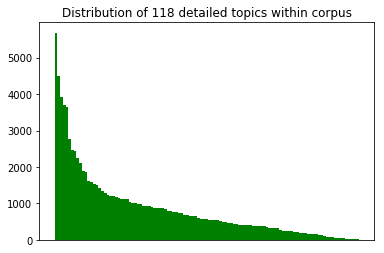
\includegraphics[width=.49\linewidth]{TrainLabels118}}~\belowbaseline[0pt]{ 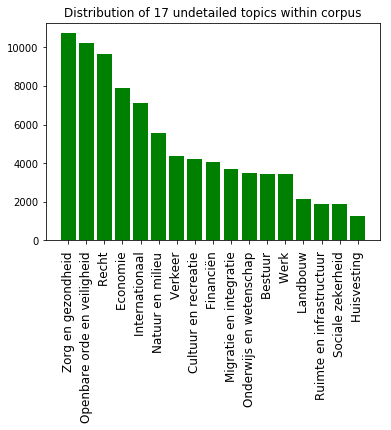
\includegraphics[width=.49\linewidth]{TrainLabels17}}
%		\caption{Distribution of labels within the parlement data}
%		\label{fig:distributiontopics}
%	\end{center}
%\end{figure}
%
%Each question-answer pair is annotated with a number of labels. Each of the labels then consists of two levels of detail; it has one of the 17 undetailed labels, such as law or education, and one of the 118 more detailed labels, such as criminal law or primary education. Figure \ref{fig:distributiontopics} shows the distributions of labels within the dataset and figure \ref{fig:LabelAmount} shows how many labels each document contains.\\
%
%\begin{figure}[H]
%	\centering
%  	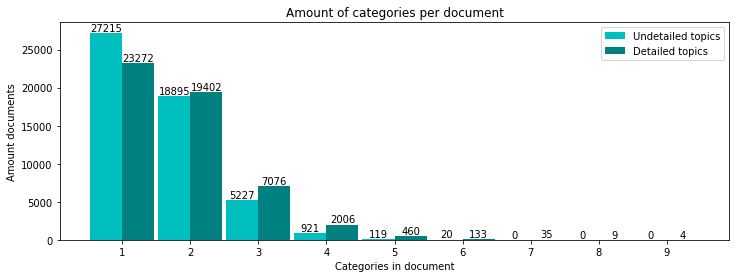
\includegraphics[width=.9\linewidth]{TrainAmountLabels}
%  	\caption{Amount of labels per document}
%  	\label{fig:LabelAmount}
%\end{figure}
%
%The questions are collected from www.zoek.officielebekendmakingen.nl with a scraper and the set consist of all question asked from 2001 to 2017. This means all of the labels have been discussed in many debates and varieties. Moreover, the documents vary on length as can be seen in Figure \ref{fig:WordAmount} and which politicians have asked and answered these questions.\\
%
%\begin{figure}[H]
%	\centering
%  	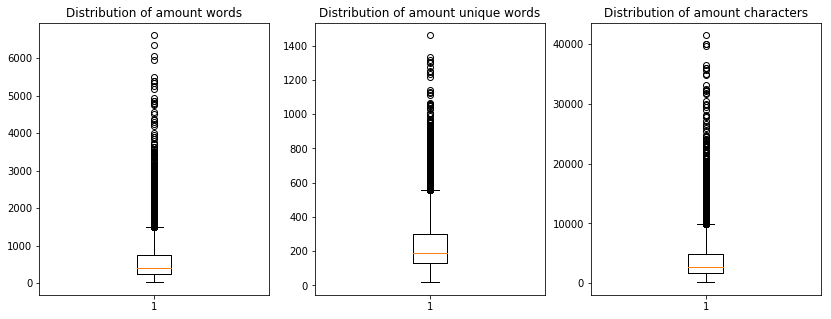
\includegraphics[width=.9\linewidth]{TrainAmountWords}
%  	\caption{Box plots of the amount of words, unique words and characters within the train data.}
%  	\label{fig:WordAmount}
%\end{figure}
%
%The second part of the data is retrieved from www.zoek.openraadsinformatie.nl, which contains documents of Dutch municipalities. These municipality documents consist of all kind of documents produced within municipalities, such as items on the agenda and notifications of commissions. These too have a great variety in content which ranges from discussion about local infrastructure to the re-allocation of local sport clubs. \\

%\begin{figure}[H]
%	\begin{center}
%		\includegraphics[width=.9\linewidth]{MunLabels17}
%		\caption{Distribution of labels within the municipality data}
%		\label{fig:MunLabels17}
%	\end{center}
%\end{figure}
%
%Large amounts of municipality data can be collected, but for this research just 25000 documents were used. Around 500 of these document were manually labeled using the taxonomieBeleidsagenda, which is the same taxonomy used for the Dutch parliament. However, the detailed labels have not been assigned, as these are too specific for untrained annotators. Similar to the training set, an overview of the label distribution, amount of labels and length of the labeled documents are visualized within Figures \ref{MunLabels17},\ref{MunAmountLabels} and \ref{MunAmountWords}. \\

%\begin{figure}[H]
%	\centering
%  	\includegraphics[width=.9\linewidth]{MunAmountLabels}
%  	\caption{Amount of labels per municipality document}
%  	\label{fig:MunAmountLabels}
%\end{figure}
%
%\begin{figure}[H]
%	\centering
%  	\includegraphics[width=.9\linewidth]{MunAmountWords}
%  	\caption{Box plots of the amount of words, unique words and characters within the municipality data.}
%  	\label{fig:MunAmountWords}
%\end{figure}

%This research adds to the existing architectures in its method to deal with variable document sizes instead of merely padding and cutting sentences to the input size. Two possibilities have been examined; Firstly, the sentences are split into multiple smaller parts. Each of these individual parts of the sentence are classified individually. Then these predictions aggregated into one prediction, either by summing or using the max value. Then once again these predictions are rounded per label to create a prediction. All the parameters of the basic version of CNN are listed in Table \ref{ParametersCNN}.\\
%The second implementation attempts to fix the length discrepency within the embedding stage. The documents are all split in an equal number pieces. These pieces are then embedded using the Par2Vec embeddings \cite{le2014distributed}, which employs a pre-trained embedding space. This method ensures that all the documents have an equal input size for the network, however, for some documents the embeddings represent multiple words or even entire paragraphs. Similarly to the other classifiers, multiple parameters are tested such as input-size, static and non-static initialization and filter sizes. \\ 

%\subsection{Experiments}
%The various algorithms are evaluated on the basis of two test-sets, both from a different source of data as explained in section \ref{subsec:data}. The first experiment is carried out on the data with question of the Dutch parlement. This set is split into three parts of respectively 70, 20 and 10 percent of the data. The models are firstly trained on 70 percent of the data. Then, the optimal hyperparameters, such as the decision threshold, are chosen by evaluating the performance on the 20 percent of the data. When these parameters have been selected, the final versions is tested with the last 10 percent of the data. This experiment is conducted twice, using both the data with 17 and 118 different topics. Using different amount of topics shows how well algorithms perform depending on the detail of the topics.\\
%Within the second experiment the transfer between different datasets is specifically important. The model is trained on 80 percent of the parlement-data and the remaining parlement data is used as validation data to select the optimal parameters. However, this model is evaluated using the manually labelled dataset of the Dutch municipalities in order to see how well the models transfer to another dataset. In contrast to the first experiment this experiment is merely conducted with 17 topics, as the municipality data is only classified that way.\\
%Success in both experiments is measured using the micro-average F1-score, which balances the precision and recall of the prediction. However, in addition to the F1-scores also confusion matrices are used in order to evaluate what kind of errors are made. Lastly, properties of documents that are missclassified are evaluated per algorithm to better understand how the algorithms perform on specific types of documents. 


%Hoe je je vraag gaat beantwoorden.
%
%
%Dit is de langste sectie van je scriptie. 
%
%Als iets erg technisch wordt kan je een deel naar de Appendix verplaatsen. 
%
%Probeer er een lopend verhaal van te maken.
%
%Het is heel handig dit ook weer op te delen nav je deelvragen:
%
%\subsubsection{RQ1}
%
%\subsubsection{RQ2}